\subsubsection{FAT-16文件系统使用测试}
将上述实现的FAT-16文件系统编译后运行,测试结果如下:
\begin{figure}[H]
    \centering
    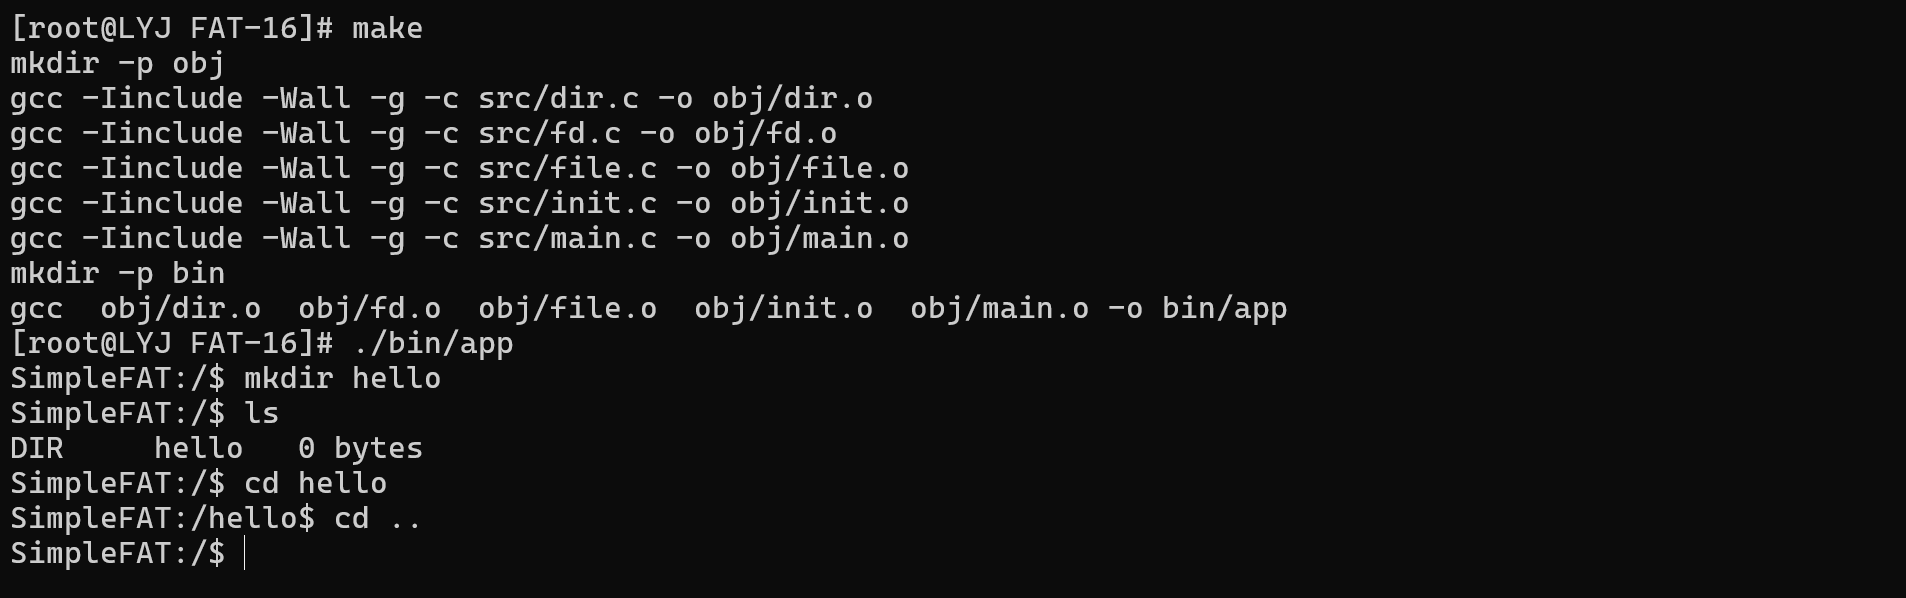
\includegraphics[width = 1\textwidth]{figure/mkdir_cd.png}
    \caption{创建文件夹和切换目录}
\end{figure}
\begin{figure}[H]
    \centering
    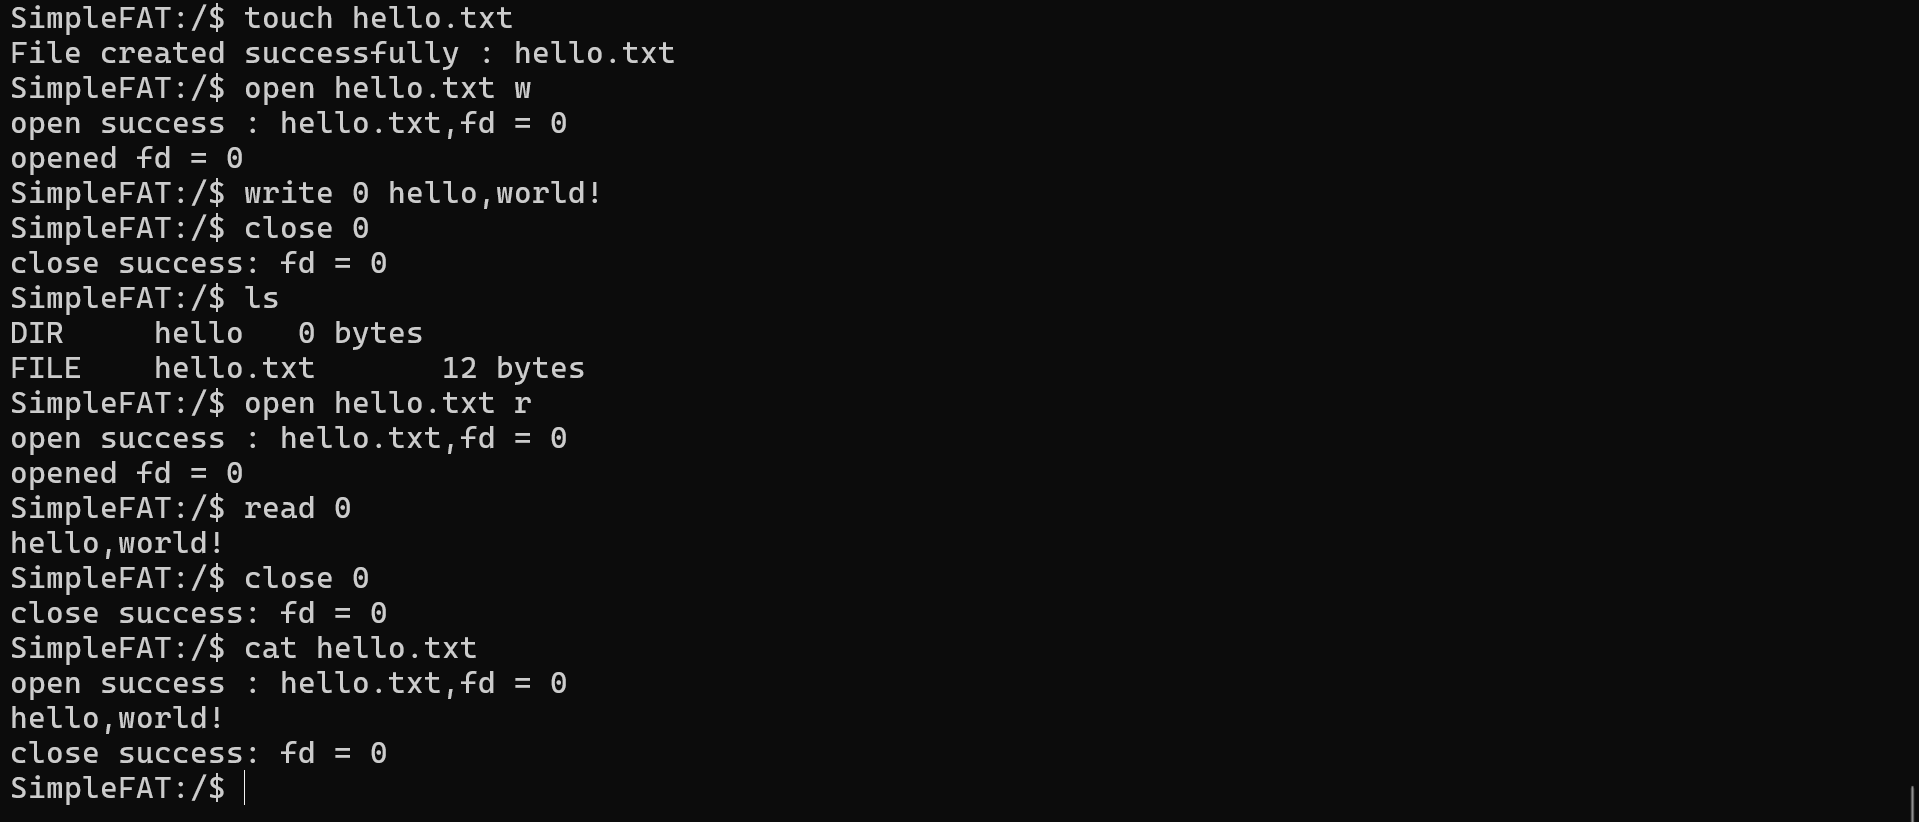
\includegraphics[width = 1\textwidth]{figure/touch_read_write.png}
    \caption{创建文件和读写文件}
\end{figure}

\begin{figure}[H]
    \centering
    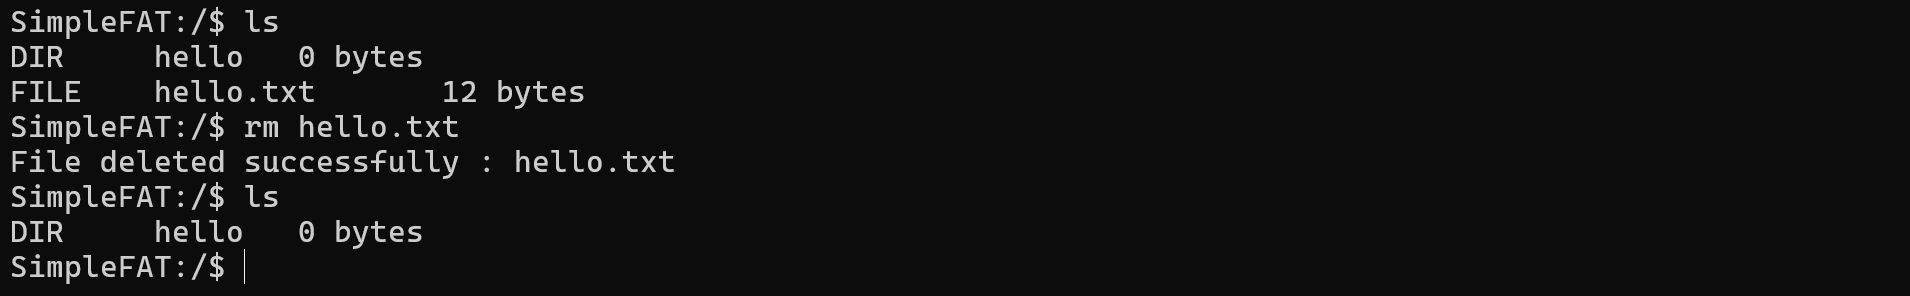
\includegraphics[width = 1\textwidth]{figure/delete.png}
    \caption{删除文件}
\end{figure}
从上述测试结果截图可以看到,该FAT-16文件系统能成功实现基于内存的单进程文件系统,正确完成了mkdir、ls、cd、touch、cat、open、read、write、close、rm等功能,任务一成功完成。

\subsection{任务一函数汇总}
下表对任务一实现的所有主要函数进行汇总,以便对照查阅。

\begin{table}[H]
\centering
\caption{任务一主要函数汇总}
\label{tab:task1_summary}
\resizebox{\textwidth}{!}{%
\begin{tabular}{|c|c|c|c|}
\hline
\textbf{函数名} & \textbf{功能} & \textbf{实现方法} & \textbf{关键数据结构} \\
\hline
\texttt{init\_fs()} & 初始化文件系统 & 清零Disk/FAT/Directory数组,初始化根目录项 & Disk[], FAT[], Directory[] \\
\hline
\texttt{init\_fd\_table()} & 初始化文件描述符表 & memset清零,dir\_index置为-1 & FDTable[] \\
\hline
\texttt{mkdir()} & 创建目录 & 遍历Directory找空闲项,设置目录名/类型/父目录索引 & Directory[] \\
\hline
\texttt{ls()} & 列出当前目录内容 & 遍历Directory,匹配parent==current\_dir,打印类型/名称/大小 & Directory[], current\_dir \\
\hline
\texttt{cd()} & 切换当前目录 & 修改current\_dir,支持/、..、下级子目录名 & Directory[], current\_dir \\
\hline
\texttt{fs\_create()} & 创建文件 & 在Directory中找空闲项,设置文件名/类型/父目录索引 & Directory[] \\
\hline
\texttt{fs\_open()} & 打开文件 & 遍历Directory查找文件→在FDTable中分配空闲表项→返回fd & Directory[], FDTable[] \\
\hline
\texttt{fs\_close()} & 关闭文件 & 验证fd有效性→将FDTable对应表项清零 & FDTable[] \\
\hline
\texttt{fs\_read()} & 读取文件内容 & 从offset所在块开始,沿FAT链逐块memcpy到buffer & Disk[], FAT[], FDTable[] \\
\hline
\texttt{fs\_write()} & 写入文件内容 & 确保FAT链有足够块→从offset逐块写入data→更新文件大小 & Disk[], FAT[], FDTable[] \\
\hline
\texttt{fs\_delete()} & 删除文件 & 沿FAT链释放所有块(FAT标记为0),目录项标记为未使用 & Directory[], FAT[] \\
\hline
\texttt{fs\_seek()} & 设置读写偏移 & 验证fd和offset有效性→更新FDTable中offset字段 & FDTable[] \\
\hline
\end{tabular}%
}
\end{table}
